\documentclass{beamer}
\usepackage[english, russian]{babel}
\usepackage[T2A]{fontenc}
\usepackage[utf8]{inputenc}
\usepackage{indentfirst}
\usepackage{amsmath, amsfonts, amssymb, amsthm, mathtools}
\usepackage[export]{adjustbox}
\usepackage{graphicx} 
\graphicspath{ {./images/} }

\usepackage{subcaption}
\usepackage{verbatim}

\usepackage{minted}{\setlength{\parskip}{0pt}}

\usepackage{hyperref}

\hypersetup{
    colorlinks=true,
    linkcolor=blue,
    filecolor=magenta,      
    urlcolor=black,
    pdftitle={Overleaf Example},
    pdfpagemode=FullScreen,
    }


\title{Лабораторная работа № 15. \\ Настройка сетевого журналирования}
\author{Данила Стариков \\ НПИбд-02-22}
\institute{Российский университет дружбы народов имени Патриса Лумумбы}
\date{2024}

\begin{document}

\frame{\titlepage}

\begin{frame}
\frametitle{Цель работы}
\begin{itemize}
    \item Получение навыков по работе с журналами системных событий.
\end{itemize}
\end{frame}

\begin{frame}
\frametitle{Настройка сервера сетевого журнала}
    \centering
    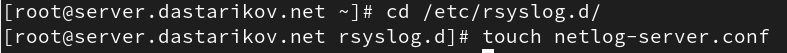
\includegraphics[width=\textwidth]{../images/image01.png}
    \captionof{figure}{Создание файла конфигурации для сетевого хранения журналов на сервере.}
\end{frame}


\begin{frame}
\frametitle{Настройка сервера сетевого журнала}
    \centering
    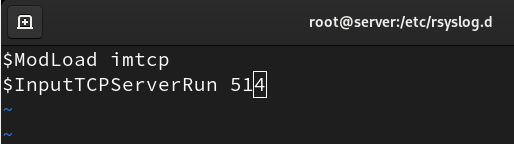
\includegraphics[width=\textwidth]{../images/image02.png}
    \captionof{figure}{Включение приема записей журнала по TCP-порту 514.}
\end{frame}


\begin{frame}
\frametitle{Настройка сервера сетевого журнала}
    \centering
    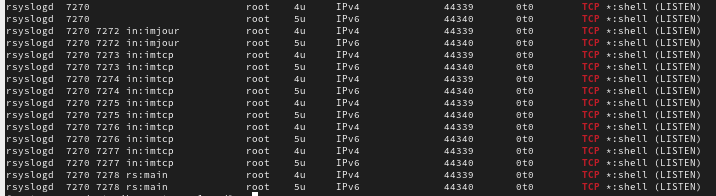
\includegraphics[width=\textwidth]{../images/image03.png}
    \captionof{figure}{Проверка прослушиваемых rsyslog портов.}
\end{frame}


\begin{frame}
\frametitle{Настройка сервера сетевого журнала}
    \centering
    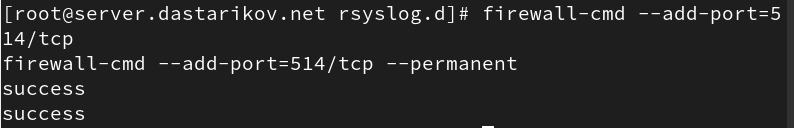
\includegraphics[width=\textwidth]{../images/image04.png}
    \captionof{figure}{Настройка межсетевого экрана для приема сообщений по TCP-порту 514.}
\end{frame}


\begin{frame}
\frametitle{Настройка клиента сетевого журнала}
    \centering
    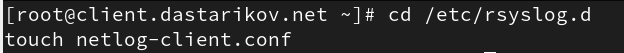
\includegraphics[width=\textwidth]{../images/image05.png}
    \captionof{figure}{Создание файла конфигурации сетевого хранения журналов на клиенте.}
    \centering
    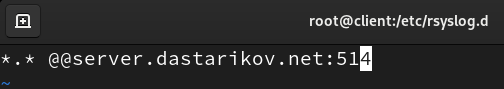
\includegraphics[width=\textwidth]{../images/image06.png}
    \captionof{figure}{Включение перенаправления сообщений журнала на сервер через TCP-порт 514.}
    \centering
    
\includegraphics[width=\textwidth]{../images/image07.png}
    \captionof{figure}{Перезапуск службы rsyslog.}
\end{frame}


\begin{frame}
\frametitle{Просмотр журнала}
    \centering
    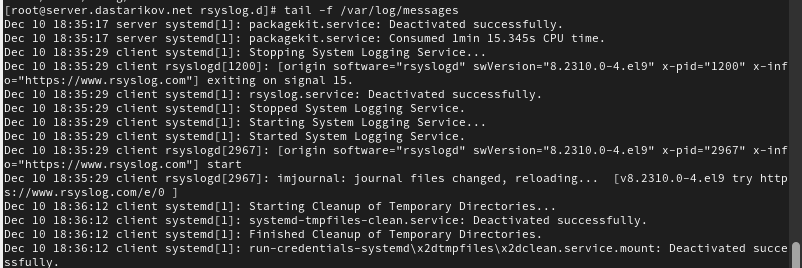
\includegraphics[width=\textwidth]{../images/image08.png}
    \captionof{figure}{Просмотр файла журнала на сервере.}
\end{frame}


\begin{frame}
\frametitle{Просмотр журнала}
    \centering
    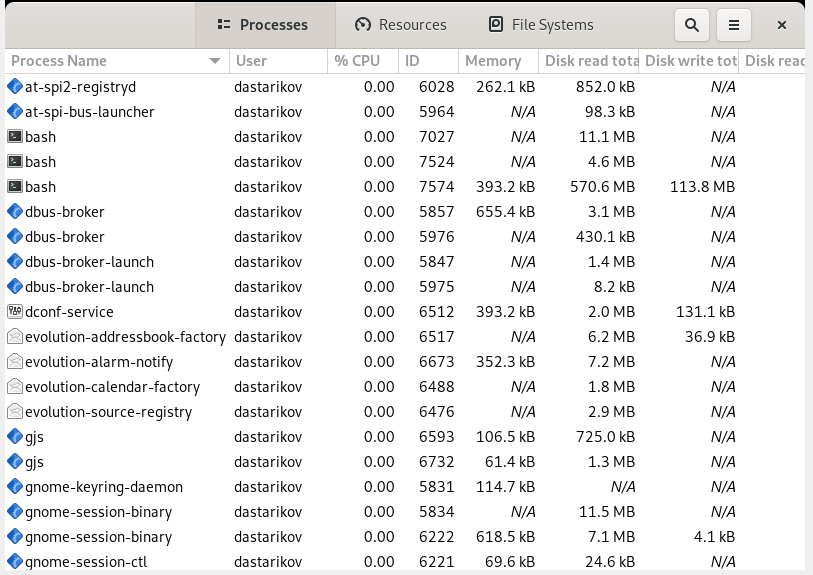
\includegraphics[width=\textwidth]{../images/image09.png}
    \captionof{figure}{Просмотр журнала на клиенте через графическую программу.}
\end{frame}


\begin{frame}
\frametitle{Просмотр журнала}
    \centering
    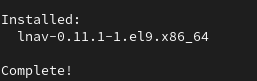
\includegraphics[width=\textwidth]{../images/image10.png}
    \captionof{figure}{Установка просмотрщика журналов системных сообщений на сервер.}
\end{frame}


\begin{frame}
\frametitle{Просмотр журнала}
    \centering
    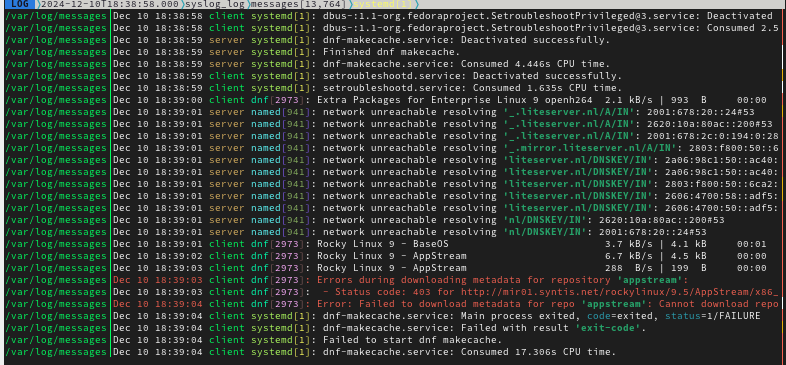
\includegraphics[width=\textwidth]{../images/image11.png}
    \captionof{figure}{Просмотр общих логов на сервере.}
\end{frame}


\begin{frame}
\frametitle{Просмотр журнала}
    \centering
    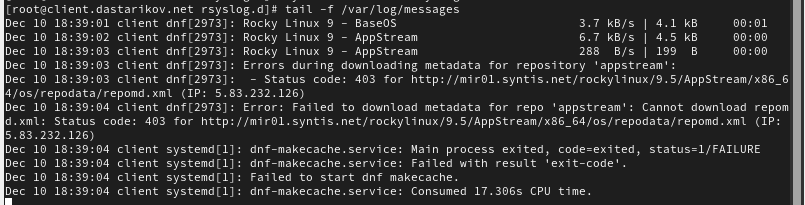
\includegraphics[width=\textwidth]{../images/image11a.png}
    \captionof{figure}{Логи на клиенте.}
\end{frame}


\begin{frame}
\frametitle{Внесение изменений в настройки внутреннего окружения виртуальных машин}
    \centering
    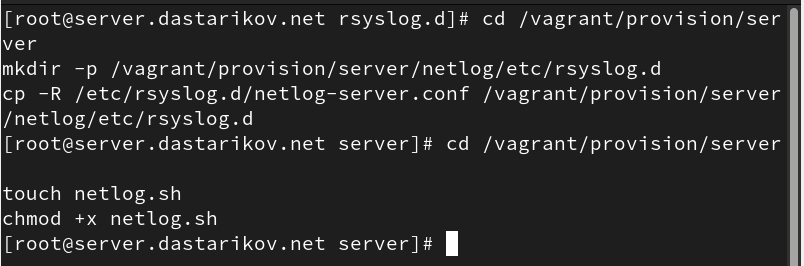
\includegraphics[width=\textwidth]{../images/image12.png}
    \captionof{figure}{Создание каталога для настройки внутреннего окружения на сервере.}
\end{frame}


\begin{frame}
\frametitle{Внесение изменений в настройки внутреннего окружения виртуальных машин}
    \centering
    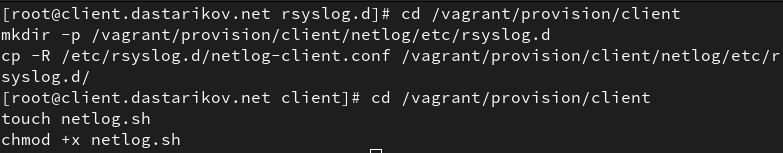
\includegraphics[width=\textwidth]{../images/image13.png}
    \captionof{figure}{Создание каталога для настройки внутреннего окружения на клиенте.}
\end{frame}


\begin{frame}
\frametitle{Выводы}
\begin{itemize}
    \item В результате выполнений лабораторной работы получили навыки настройки сетевого хранения журналов системных событий.
\end{itemize}
\end{frame}
\end{document}
